\documentclass[a4paper]{article}

\usepackage[margin=80pt]{geometry}
\usepackage[ngerman]{babel}

\usepackage[scaled]{helvet}
\renewcommand{\familydefault}{\sfdefault}
\usepackage[T1]{fontenc}

\usepackage[hidelinks]{hyperref}
\hypersetup{colorlinks=false}

\usepackage{enumitem}
\setlist{nosep}

\usepackage[utf8]{inputenc}
\usepackage{graphicx}
\usepackage{enumitem}

% Package und Einstellungen für Java-Code-Darstellung
\usepackage{listings}
\usepackage{color}
\definecolor{dkgreen}{rgb}{0,0.6,0}
\definecolor{gray}{rgb}{0.5,0.5,0.5}
\definecolor{mauve}{rgb}{0.58,0,0.82}
\lstset{frame=tb,
	language=Java,
	aboveskip=3mm,
	belowskip=3mm,
	showstringspaces=false,
	columns=flexible,
	basicstyle={\small\ttfamily},
	numbers=none,
	numberstyle=\tiny\color{gray},
	keywordstyle=\color{blue},
	commentstyle=\color{dkgreen},
	stringstyle=\color{mauve},
	breaklines=true,
	breakatwhitespace=true,
	tabsize=3
}

\title{\textbf{SWDE - Software Development\\
Zusammenfassung FS 2019}}
\date{\today}
\author{Maurin D. Thalmann}

\begin{document}
	\pagenumbering{gobble}
	\maketitle
	\newpage
	\pagenumbering{arabic}
	\tableofcontents
	\newpage
	
	\section{Buildautomatisation}
	
		\subsection{Sie kennen die Vorteile eines automatisierten Buildprozesses}
			\begin{itemize}
				\item Automatisierter Ablauf, keine Interaktion mehr benötigt
				\item Reproduzierbare Ergebnisse
				\item lange Builds können auch über Nacht laufen
				\item Unabhängig von Entwicklungsumgebung
			\end{itemize}
		
		\subsection{Sie können verschiedene Beispiele von Buildwerkzeugen benennen}
			\begin{description}
				\item[Make] (für C/C++ Projekte), Urvater der Build Tools, \\
				hohe Flexibilität, gewöhnungsbedürftige Syntax
				\item[Ant] Java mit XML
				\item[Maven] Java mit XML
				\item[Buildr] Ruby-Script
				\item[Gradle] Groovy Script mit DSL
				\item[Bazel] Java mit Python-like Scripts
			\end{description}
		
		\subsection{Sie beherrschen die Anwendung eines ausgewählten Buildwerkzeuges (Apache Maven)}
		Beherrschen muss man es selber, es kann entweder aus der Shell (Terminal/Konsole) verwendet werden oder aus den integrierten Funktionen in der IDE selbst.
		
		\subsection{Sie sind mit den wesentlichen Konzepten von Apache Maven vertraut}
		Deklaration des Projektes in XML, zentrales Element pro Projekt ist das \textbf{Project Object Model (POM)}, welches Metainformationen, Plugins und Dependencies definiert. 
		Basiert auf einem globalen, binären Repository. Plugins werden durch Dependencies dynamisch ins lokale Repository geladen (\$HOME/.m2/repository)\\
		Bei einem Buildprozess durchläuft ein Projekt einen Lifecycle mit folgenden Phasen:\\
		\begin{description}
			\item[validate] validiert Projektdefinition
			\item[compile] Kompiliert die Quellen
			\item[test] Ausführen der Unit-Tests
			\item[package] Packen der Distribution
			\item[verify] Ausführen der Integrations-Tests
			\item[install] Deployment im lokalen Repository
			\item[deploy] Deployment im zentralen Repository
		\end{description}

	\newpage
	\section{Modularisierung - Module, Komponenten, Schnittstellen}
	
	\subsection{Sie wissen, was unter dem Begriff Modularisierung zu verstehen ist}
	\textit{«Ein grosses Ganzes in mehrere, sich abgeschlossene Einheiten (Module) aufteilen»} \\
	Flexible Zusammenstellung, Durchführung und Prüfung der einzelnen Module. 
	Zwischen den Modulen können aber auch Abhängigkeiten bestehen.
	
	\subsection{Sie kennen die Begriffe Modul, Library, Komponenten und Schnittstelle auf der Ebene des Softwaredesigns}
	\textbf{Kleinste Einheit:} Klasse (Methoden/Daten/Attribute) $\leftrightarrow$ \textbf{Grösste Einheit:} vollständiges Softwaresystem
	\begin{description}
		\item[Modul] In sich abgeschlossene und austauschbare Einheiten, \\
		soll nur über seine Schnittstellen verwendet werden können $\rightarrow$ lose Kopplung; \\
		Starke Kohäsion (möglichst in sich abgeschlossene Aufgabe erfüllen) $\rightarrow$ Information Hiding
		\item[Schnittstelle] lässt Module untereinander interagieren / austauschen
		\item[Komponente] strengere Form eines Moduls
		\item[Library] Eine Sammlung thematisch zusammengehörender Funktionen (z.Bsp. Kalendermodul, Trigonometriemodul, etc.)
	\end{description}
	\textit{Die einzelnen Begriffe werden in einem späteren Lernziel ausführlicher beschrieben.}
	
	\subsection{Sie können die Begriffe auf verschiedenen Abstraktionsebenen in einen sinnvollen Zusammenhang und Kontext setzen}
	\begin{description}
		\item[Kopplung] Ausmass der Kommunikation zwischen Modulen (Abhängigkeit zw. Modulen)
		\item[Kohäsion] Ausmass der Kommunikation innerhalb eines Moduls (interner Zusammenhalt)
		\item[Ziel] $\rightarrow$ Maximierung der Kohäsion, Minimierung der Kopplung
	\end{description}
	\begin{description}
		\item[Gruppierung] Modulen mit gemeinsamen Eigenschaften als Gruppe handhaben. \\
			\textit{Beispiel}: Modul für Datenexport in versch. Formate
		\item[Hierarchie (Rekursiv)] Modul fasst mehrere (Sub-) Module zu einem zusammen. \\
			\textit{Beispiel}: Persistenzmodul als Datenspeicher mehrerer Entitäten
		\item[Geschichtet] Modul(-gruppen) können logische Kette bilden, die vertikal als Schichten abgebildet werden. \\
			\textit{Beispiel}: Schichtenarchitektur, OSI-Referenzmodell, etc.
	\end{description}
	
	\newpage
	\subsection{Sie sind in der Lage ein System zu analysieren und darin sinnvolle Module zu identifizieren}
	
	\subsubsection{Modul}
	\textbf{\underline{Kriterien für Entwurf von Modulen:}}\\
	\textbf{Zerlegbarkeit / Dekomposition}\\
	möglichst unabhängig voneinander, können einzeln genutzt/wiederverwendet werden\\
	\textbf{Kombinierbarkeit}\\
	sollen in anderem Umfeld wieder einsetzbar sein \\
	\textit{(Zerlegbar, um auf andere Art wieder kombiniert werden zu können)}\\
	\textbf{Verständlichkeit}\\
	unabhängig und in sich abgeschlossen verständlich sein, kann aber trotzdem hohe Komplexität erreichen.\\
	\textbf{Stetigkeit / Stabilität / Kontinuität}\\
	Struktur soll sich nicht stetig verändern, Aufteilung soll robust gegenüber Änderungen sein. Änderungen sollen sich auf eine minimale Anzahl Module beschränken.\\
	\newline
	\textbf{\underline{Arten von Modulen:}}\\
	\textbf{Bibliothek/Library:} beschrieben unter Kapitel 2.2\\
	\textbf{Abstrakte (komplexe) Datentypen:} Modul implementiert neuen komplexen Datentyp und stellt darauf definierte Operationen zur Verfügung (Bsp. Komplexe Zahlen, Koordinatendarstellung, etc.)\\
	\textbf{Modellierung/Abstraktion physischer Modelle:} Modul abstrahiert reales, physisch existierendes System (z.Bsp. Sensor, Gerätetreiber, Anzeigemodul, etc.)\\
	\textbf{Modellierung/Abstraktion logisch-konzeptioneller Systeme:} Modul abstrahiert ein nur rein logisch existierendes System und macht es für eine höhere Abstraktionsebene nutzbar (z.Bsp. Grafikmodule, Datenbankmodule, Messaging, GUI-Module, etc.)\\
	\newline
	\textbf{\underline{Definition eines Moduls:}}\\
	\textbf{Verhalten:} Funktionalität des Moduls?\\
	\textbf{Export:} Was bieten wir, Schnittstelle, um das Verhalten des Moduls für andere Module verfügbar zu machen.\\
	\textbf{Import:} Was brauchen wir, von welchen Schnittstellen ist das Modul evtl. abhängig? (Dependencies)\\
	\newline
	\textbf{\underline{Herausforderung bei Modulen:}} \\
	\textbf{Basiskonzepte:} Hohe Kohäsion, lose Kopplung, starke Datenkapselung \& Information Hiding\\
	\textbf{Vier Kriterien:} Zerlegbarkeit, Kombinierbarkeit, Verständlichkeit \& Stetigkeit\\
	\textbf{Verschiedene Arten:} Bibliotheken, abstrakte Datentypen, physische / logische Modelle, Komponenten, etc.

	\subsubsection{Komponente}
	\begin{quote}
		\textit{Eine Softwarekomponente ist ein Softwareelement, das zu einem
bestimmten \textbf{Komponentenmodell} passt und entsprechend
einem Composition Standard ohne Änderungen mit anderen
Komponenten verknüpft und ausgeführt werden kann.}
	\end{quote}
	Eine \textbf{Komponente} erfüllt strengere Kriterien als ein Modul und benötigt meist einen \textbf{Kontext}.
	Komponenten bedienen sich spezifischer Laufzeitumgebungen (z.Bsp. Container) in welche die Komponenten integriert (installiert, deployed, etc.) werden und dort lauffähig sind (Container stellen den Komponenten Basisdienste z.Bsp. für Lifecycle und Kommunikation bereit)\\
	Komponenten können teilweise \textbf{dynamisch zur Laufzeit} ergänzt/entfernt/ausgetauscht werden
	\\ \indent $\rightarrow$ «Hot-Deployment» / Plugin-Mechanismen\\
	Komponenten bieten Funktionalität an und sind von Funktionalität des eingesetzten Komponentenmodells (Framework/Produkt) \textbf{abhängig}.\\
	
	\newpage
	\noindent
	\textbf{Komponentenmodelle}: konkrete Ausprägungen des Paradigmas der komponentenbasierten Entwicklung in Form eines Standards, Frameworks, Produktes. Schnittstellen für Interaktion und Komposition von Komponenten festlegen: wie kommunizieren Komponenten untereinander/mit dem Container Idealerweise: Komponentenmodell unabhängig von Gremium standardisiert (kann somit in unterschiedlichen Ausprägungen von versch. Herstellern implementiert/genutzt werden)
	\begin{quote}
			\textbf{Beispiele}: Microsoft DCOM/ActiveX/.NET Remoting Services (WCF), CORBA (Common Object Request Broker Architecture), Enterprise Java Beans, OSGi (Open Services Gateway initiative / Alliance)
	\end{quote}
	\textbf{Komponente} wird wie Modul über \textit{Verhalten, Export, Import} definiert. \\
	Zusätzlich wird ein \textbf{Kontext} verlangt: definiert notwendige Rahmenbedingungen, die für Betrieb der Komponente notwendig sind.
	
	\subsubsection{Schnittstelle}
	Schnittstellen werden konsequent für die kontrollierte Kommunikation zwischen Modulen oder Komponenten verwendet. \textbf{Vorteile} davon:
	\begin{itemize}
		\setlength\itemsep{0em}
		\item Schnittstelle ist einfach verständlich, einfacher als die Implementierung.
		\item Schnittstellen helfen Abhängigkeiten zu reduzieren, vermeiden Abhängigkeiten zur Implementierung.
		\item Schnittstellen erleichtern Wiederverwendung.
	\end{itemize}
	Beziehungen zwischen einzelnen Teilen einer Software werden über Schnittstellen realisiert. Module konzentrieren sich auf ihre lokalen Probleme, Architektur definiert und hält Fäden (Beziehungen) des Systems zusammen.\\
	Schnittstellen sollen minimal und schmal sein $\rightarrow$ aussagekräftige Methoden, präzis typisierte Parameter, \textbf{Methoden} sollen möglichst:
	\begin{itemize}
		\setlength\itemsep{0em}
		\item keine Überschneidungen haben
		\item keine globalen Daten verwenden
		\item statuslos (stateless) sein
	\end{itemize}
	\textbf{Service}: abstrahierte Schnittstelle, definiert sich primär über Fachlichkeit, dahinterliegende Technik idealerweise vollständig isoliert (Bsp. Webservice, wird über Web-Protokolle angeboten und abstrahiert die Implementation [Plattform, Sprache, Technologie] vollständig) \\
	\textbf{API}: \textit{(Application Programming Interface)}, technisch orientierte Schnittstelle, welche die Anbindung einer Komponente auf Quellcodeebene definiert (Bsp. JDBC [Java Database Connectivity], einheitliche Schnittstelle zur Kommunikation mit versch. DBMS) \\
	Ebene \textbf{Objektorientiertes Design}: Schnittstelle = Java Interface \\
	Ebene \textbf{Modularisierung}: Schnittstelle = logische Zusammenfassung versch. Artefakte (Klassen, Interfaces, Konfigurationsdateien, Doku etc.)
	
	\newpage
	\subsection{Sie kennen verschiedene organisatorische und technische Varianten um eine sinnvolle Modularisierung in der Entwicklung und im Deployment einzusetzen}
	\subsubsection{Java 8}
	Module/Komponenten mit Klassen und Interfaces realisiert, Deployment meist als JAR. 
	Klassen können sich an «Java Bean Spezifikation» halten \\ 
	\indent $\rightarrow$ Default-Konstruktor, Setter/Getter, PropertyChange, Serialisierbar, etc. \\
	Schnittstellen mit Java-Interfaces (zu class-Dateien kompiliert) \\
	Komplexere Schnittstellen: mehrere Interfaces in Package zusammenfassen \\
	Java 1.8 unterstützt selber keine Modularisierung \\
	Information Hiding (einzelne Elemente vor Zugriff schützen) durch Packages, Sichtbarkeiten und Import, ermöglicht Zusammenfassen von Klassen/Interfaces in Gruppen, aber keine explizite Möglichkeit, Exports \& Dependencies zu deklarieren \\
	manifest.mf enthält Infos zu Identifikation, Herkunft und Version \\
	Schnittstellen in getrennten JAR’s (Modulen) verteilen $\rightarrow$ einfacher Austausch unterschiedlicher Implementationen \\
	\textit{Workaround}: Namenskonventionen und hohe Disziplin \\
	
	\subsubsection{Java 9}
	Modularisierung möglich, drei Ziele im Vordergrund:
	\begin{itemize}
		\setlength\itemsep{0em}
		\item \textbf{Reliable Configuration:} \\
		fehleranfälligen Classpath durch auf Modul-Abhängigkeiten basierenden Modul-Path ablösen
		\item \textbf{Strong Encapsulation:} \\
		Modul definiert explizit sein öffentliches API. 
		Auf alle restlichen Klassen ist von aussen kein Zugriff mehr möglich (auch wenn public).
		\item \textbf{Scalable Platform:} \\
		Java-Plattform selber wurde modularisiert, so können für Anwendungen individuell angepasste, schlankere Runtime-Images gebaut werden.
	\end{itemize}
	Weiteres zu Modularisierung in Java 9:
	\begin{itemize}
		\setlength\itemsep{0em}
		\item Java-Packages neu in Modulen zusammenfassbar (zusätzliche Strukturebene in der Dateiablage, eindeutige Namensgebung analog zu Packages)
		\item Pro Modul wird ein \textit{module-info.java} definiert (explizite Definition von Imports/Exports/Abhängigkeiten)
		\item Start einer Applikation: Laufzeitprüfung wird ausgeführt, ob alle notwendigen Komponenten vorhanden sind.
		\item Ende der «JAR-Hell»: Neues Format \textit{jmod}, Class-Path wird durch Modul-Path abgelöst
		\item Vollständig rückwärtskompatibel
	\end{itemize}

\newpage
\section{Dependency Management}

	\subsection{Sie haben ein grundsätzliches Verständnis von Dependency Management}
	
	\paragraph{Dependency Management}
	
	Beschreibt die Organisation und Techniken für Umgang mit Abhängigkeiten mi anderen Modulen.\\
	\textit{("Modul" hier vereinfacht als Überbegriff für Package / Library / Bundle / Komponente verwendet)}\\
	Abhängigkeiten können auf \textbf{interne} (Modul aus demselben Projekt) oder \textbf{externe} (Dritt-Modul aus anderem Projekt / Organisation) Module bestehen.
	Abhängigkeiten werden typisch in binärer / kompilierter Form aufgelöst, wozu Binärrepositories und Packagemanager(-tools) eingesetz werden.\\
	Allen Systemen / Repositories ist gemeinsam:
	\begin{itemize}
		\item Zentrale Ablage auf einem (oder mehrere) Server
		\item standartisiertes Format
		\item zusätzliche Metainformationen
		\item typisch mit Abhängigkeiten (Dependencies) versehen
		\item Sicherung der Konsistenz (bspw. über Hash-Mechanismen)
		\item geregelte Zugriffsprotokolle
		\item Suchmöglichkeiten u.v.m.
	\end{itemize}
	\vspace{1em}
	Beispiele von populären Systemen / Repositories für DM und PM:
	\begin{description}
		\item[NuGet] Package Manager für .NET-Plattform
		\item[apt] Advanced Packaging Tool - Packetverwaltung für Linux
		\item[Yum] Yellowdog Updater, Modified - Packetverwaltung für Linux
		\item[P2] OSGi-basiertes Komponentensystem
		\item[npm] Node Packet Manager für JavaScript / node.js
		\item[Gems] Packetmanager Ruby
	\end{description}
	
		\subsubsection{Maven Repository}
		
		\begin{itemize}
			\item Verschiedene öffentliche Repos \textbf{(OSS)}: Maven Central, JFrog JCenter (BinTray)
			\item Keine Schreibrechte auf öffentliche Repos (nur ausgewählte Personen über definierte Prozesse)
			\item Professionelle Organisationen betreiben interne Repositories, meist als lokaler Speicher und Mirror von öffentlichen Repos, professionelle Produkte wären:\\ 
			\textit{Apache Archiva, JFrog/Artifactory, Sonatype/Nexus}
			\item Alle heruntergeladenen Artefakte vom Repo werden in lokalem Repo auf dem Rechner gespeichert (Caching) unter \texttt{\$HOME/.m2/repository}
			\item Zur Verwendung muss unter \texttt{\$HOME/.m2} die \texttt{settings.xml} Datei angepasst werden, damit die Dependencies nicht vom öffentlichen Repo geholt werden
		\end{itemize}

\newpage
	
	\subsection{Sie wissen wie am Beispiel von Java und Apache Maven das Dependency Management funktioniert}
	
	\begin{itemize}
		\item Binäre Module (kompilierte Projekte) werden unter Java typischerweise als JAR-Dateien ausgetauscht (oder EAR, WAR, RAR etc.)
		
		\item Java kennt selber kein Verfahren zur Defintion von Abhängigkeiten zwischen Modulen und deren zentraler Verwaltung\\
		(Ab Java 9: Modularisierung (Jigsaw), aber ohne Versionierung)
		
		\item Früher: JAR-Dateien von Hand in Projekte kopiert \\
		$\rightarrow$ fehleranfällig, hohe Redundanz, hoher Platzbedarf etc.\\
		Heute ist Buildsystem Maven sehr populär geworden
		
		\item Unterscheiden zwischen:
		\begin{itemize}
			\item \textbf{Format} für die zentrale Ablage der meist binären Artefakten mit Metainformationen im Repository
			\item \textbf{Werkzeug}, um Artefakte von Repos zu suchen, beziehen, deployen, ggf. auch verwalten
		\end{itemize}
	
		\item Repositoryformat Maven mittlerweile Standard, jedoch grosse Vielfalt bei Werkzeugen:
		\begin{itemize}
			\item Apache Ivy - einziges "reines" DM-Tool
			\item Apacke Maven - in Buildtool integriert, Original
			\item DM anderer Buildtools basiert ebenfalls auf Maven-Repos:\\
				Buildr, Groovy Grape, Gradle/Grails, SBT etc. 
		\end{itemize}
	\end{itemize}

		\subsubsection{Maven - Identifikation \& Dependencies}
		
		Maven Projekt identifiziert sich mit drei Attributen (\textbf{maven coordinates})
		\begin{itemize}
			\item \textbf{GroupId}:\\
					Reverse Domain Name der Organisation mit Zusatz für OE bspw. Projektgruppe\\
					Bsp: \texttt{ch.hslu.swde}
					
			\item \textbf{ArtifactId}:\\
					Name des Projekts bzw. enthaltene Module\\
					Bsp: \texttt{vereinsverwaltung-service}
					
			\item \textbf{Version}:\\
					Empfohlen: dreistellige Versionsnummer (Semantic Versioning)\\
					Bsp: \texttt{4.0.1}
		\end{itemize}
	Diese werden im \texttt{pom.xml} des Maven Projekts deklariert, damit soll eine Dependency weltweit absolut eindeutig identifiziert werden können:
	\begin{lstlisting}
<groupId>ch.hslu.swde</groupId>
<artifactId>vereinverwaltung-api</artifactId>
<version>4.0.1</version>
	\end{lstlisting}
	\noindent
	Benötigte Dependencies werden im \texttt{pom.xml} unter \texttt{<dependencies>} als ein \texttt{<dependency>}-Element eingetragen. 
	Diese werden beim Build automatisch vom Repo runtergeladen und im lokalen Repository (\texttt{\$HOME/.m2/repository}) gespeichert.
	Der Buildprozess referenziert die Artefakte dort mit entsprechendem Classpath:
	\begin{lstlisting}
<dependency>
	<groupId>ch.hslu.swde</groupId>
	<artifactId>vereinverwaltung-api</artifactId>
	<version>4.0.0</version>
	<scope>compile</scope>
</dependency>
	\end{lstlisting}
	
	\newpage
	
	\subsection{Sie sind mit den Begriffen «dependency scopes» und «transitive dependencies» vertraut und können diese erklären}
	
		\subsubsection{Dependency Scopes}
		
		\texttt{<scope>} in einer Dependency qualifiziert den Zweck und Geltungsbereich einer Dependency (wird empfohlen). 
		Abhängig von Scopes sorgt Maven für spezifische Classpaths, woraus sich eine \textit{implizite Verifikation des Designs} ergibt. 
		Maven kennt viele Scopes, die Wichtigsten sind:
		\begin{itemize}
			\item \textbf{compile}\\
					(Default) Dependency wird für Kompilation und Laufzeit des Programms benötigt
					
			\item \textbf{test}\\
					Dependency nur für Kompilation und Ausführung der Testfälle benötigt (JUnit, AssertJ, Mockito)
					
			\item \textbf{runtime}\\
					Dependency nur für Laufzeit, aber nicht für Kompilation, \\
					bspw. für dynamisch geladene Implementationen
			
		\end{itemize}
		
		\subsubsection{Transitive Dependencies}
		
		Maven bietet Feature zur Auflösung von transitiven Dependencies.
		
		\begin{figure}[!htb]
			\centering
			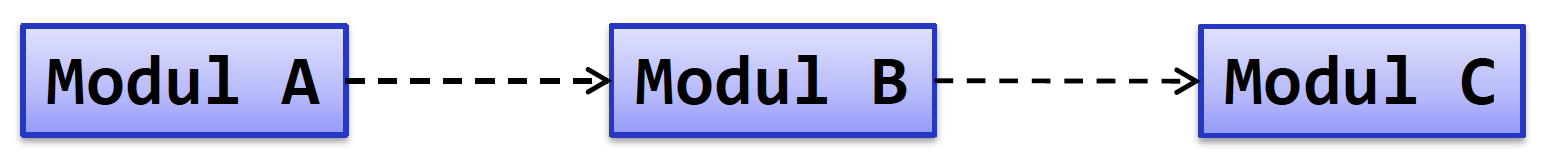
\includegraphics[keepaspectratio, height=1cm]{img/dependencymanagement/transitive_dependencies.png}
			\caption{Transitive Abhängigkeit zwischen 3 Modulen}
			\label{fig:transitive}
		\end{figure}
	
		Auflösung der Dependencies:
		\begin{itemize}
			\item \textbf{Modul A} ist von \textbf{Modul B} abhängig, dieses wiederum von \textbf{Modul C}
			\item \textbf{Modul A} ist also transitiv auch von \textbf{Modul C} abhängig
			\item Für Kompilation wird also \textbf{Model C} auch benötigt\\
			
			\item Durch direkte \& transitive Abhängigkeiten können auch Konflikte oder Zyklen auftreten.\\
			Maven erkennt und meldet diese, einfachere Konflikte können automatisch aufgelöst werden.
			\item Maven wertet die Dependencies als Graph aus, dient der Suche von Zyklen und Auflösung von Konflikten z.Bsp. über den kürzesten Pfad.
		\end{itemize}
	
	\subsection{Sie kennen das Versionskonzept und die Funktionsweise von Snapshots.}
	
	\begin{itemize}
		\item Einsatz von \textit{Semantic Versioning} wird empfohlen
		\item Einmal deployte Version kann im Optimalfall nicht mehr überschrieben werden\\
				$\rightarrow$ nachvollziehbare Buildprozesse
	\end{itemize}

			\paragraph{Semantic Versioning}
			
			\begin{itemize}
				\item \textbf{Major}-Release (\textbf{X}.x.x)\\
						Veränderungen in API, fachlicher Funktion und/oder in Konfiguration, welche zu früheren Versionen nicht kompatibel sind.
						Meist sind Anpassungen notwendig.
						
				\item \textbf{Minor}-Release (x.\textbf{X}.x)\\
						Erweiterungen in API, fachlicher Funktion oder Konfiguration, ist aber rückwärtskompatibel.
						Ohne Nutzung der Neuerungen keine Anpassungen notwendig.
						
				\item \textbf{Bugfix/Maintenance}-Release (x.x.\textbf{X})\\
						Reine Korrekturen in Änderungen oder Implementation, voll rückwärtskompatibel, keine neuen oder veränderten Funktionen.
						Direkter, sofortiger Einsatz möglich/notwendig (Bugfix)
			\end{itemize}
		
			\paragraph{Versionierung mit Snapshots}
			
			\begin{itemize}
				\item Version kann das Appendix \texttt{-SNAPSHOT} tragen.
				\item Gilt dann als erneuerbar und noch nicht stabil, sondern in Entwicklung
				\item Wird bei jedem \textbf{Build} vom Repo aufgelöst und aktualisiert
				\item Im Repo sind Snapshots mit Timestamp versehen
			\end{itemize}
	
		\subsubsection{Managed Dependencies in Multi-Modul-Projekten}
		
		\begin{itemize}
			\item Mehrere Submodule können von gleicher Dependency abhängig sein
			\item In jedem Modul sollte dieselbe Version verwendet werden
			\item \textbf{Lösung:} Im Master-POM über \texttt{dependencyManagement}-Element eine Liste an Dependencies (inkl. Version und Scope) als Baseline / Valid Version Set vordefinieren\\
			$\rightarrow$ Submodule müssen nur noch GroupId und ArtifactId angeben.
			Version und Scope werden vom Parent-POM vererbt.
			\item \textbf{\textit{Alternativ:}} Verwendung eines BOM (Bill of Material):\\
			Verschiedene Versionen werden in "virtueller" Release-Unit als "Baseline" referenziert.
			Lieferant bestimmt, welche zueinander passenden Versionen eingesetzt werden.
			Das BOM wird selber als Dependency definiert.
		\end{itemize}
	
	\subsection{Sie wissen auf welche Art Dependencies deployed werden}

	\begin{itemize}
		\item Häufigste Deployment-Art: JAR-Dateien
		\item Beispiel für ein Artefakt\\
				\texttt{ch.hslu.vsk:stringpersistor-api:4.0.1}:
			\begin{description}
				\item[POM (Metainfos)] \texttt{stringpersistor-api-4.0.1.\textbf{pom}}
				\item[JAR (Binary)] \texttt{stringpersistor-api-4.0.1.\textbf{jar}}
				\item[JavaDoc] \texttt{stringpersistor-api-4.0.1-\textbf{javadoc}.jar}
				\item[Source (bei OSS)] \texttt{stringpersistor-api-4.0.1-\textbf{sources}.jar}\\
			\end{description}
		
		\item Deployment in öffentliche Repos: sehr restriktiv\\
				$\rightarrow$ nichts mehr ändern, nichts löschen: Stabilität von Builds wahren!
		
		\item \textbf{Lösung:} nachvollziehbarer, automatisierter, verifizierbarer Release-Prozess, welcher von einem Build-Server ausgeführt wird
	\end{itemize}
	
	\newpage	
	\section{Versionskontrollsysteme - Source Code Management (SCM) / Version Control Systems (VCS)}
	
		\subsection{Sie kennen die Aufgaben eines Versionskontrollsystems und können grundlegend damit arbeiten}
		\textbf{Grundlegende Arbeit:}
		\begin{description}
			\item[checkout] lokale Arbeitskopie eines Projekts erstellen
			\item[update] Änderungen Dritter in Arbeitskopie aktualisieren
			\item[log] Bearbeitungsgeschichte eines Artefakts ansehen
			\item[diff] verschiedene Revisionen miteinander vergleichen
			\item[commit / checkin] Artefakte ins Repository schreiben $\rightarrow$ aussagekräftiger Kommentar!
		\end{description}
		\textbf{Tagging:} Revisionsstand mit Namen markieren, Marke oder Version: 1.5.2beta o.ä. Nützlich bei Release eines Produkts (aber auch meilensteine, Testversionen, Auslieferungszustände, etc.) wird unterschiedlich realisiert.\\
		\\
		\textbf{Branching:} Parallele, voneinander getrennte Entwicklungszweige (für Bugfixing, Prototypen, Tests, Experimente, nachvollziehbare Änderungsworkflows, etc.) Bei Nicht-Wegwerf-Entwicklungen später Merging möglich/notwendig.\\
		\\
		Ausschliesslich Quell-Artefakte werden verwaltet, \textbf{NIE} generierte/erzeugt Artefakte einchecken, können mit Hilfe der SCM ignoriert werden (.gitignore)
		
		\subsection{Sie kennen die verschiedenen Konzepte und Arten von Versionskontrollsystemen}
		\begin{itemize}
			\item Zentrale oder verteilte Systeme 
			\item Optimistische und pessimistische Lockverfahren 
			\item Versionierung auf Basis einer Datei, Verzeichnisstruktur oder der Änderung (changeset) 
			\item Transaktionsunterstützung (vorhanden oder nicht) 
			\item Verschiedene Zugriffsprotokolle und Sicherheitsmechanismen 
			\item Integration in Webserver (vorhanden oder nicht)
		\end{itemize}
		
		\subsection{Sie können mit verschiedenen (Client-)Werkzeugen von Versionskontrollsystemen alleine und im Team arbeiten}
		
		\begin{description}
			\item[CVS] UT-Versionskontrollsystem, stabil, wenig Fehler, einfache Anwendung, ABER nur dateibasierend, Verzeichnisstruktur nicht versioniert, unterscheidet zwischen Text- und Binärdateien, Ablage von Binärdateien platzintensiv, keine Transaktionen
			\item[Subversion] Transaktionsorieniert, versioniert ganze Verzeichnisstruktur, optimierte/effiziente Speicherung und Übertragung, Repositorystruktur frei wählbar (für Experten flexibler, für Anfänger schwieriger), Integration in Webserver möglich, aber Branching und Tagging technisch eig. Kopien/Links
			\item[git] verteiltes System, primär lokale Arbeit, beliebig viele Server/Repos möglich, auch rein lokal einsetzbar, skaliert, Integration mit zusätzlichen Web-Applikationen, erfordert aber ein solides Konzept, für Einsteiger schwierig, da sehr mächtig und viele Funktionen
		\end{description}
	
	\newpage
	\section{Testing Grundlagen}
		
		\subsection{Sie kennen die Motivation, den Sinn und den Zweck des Testens, was Sie mit Tests erreichen können und was nicht}
		
		\begin{quote}
			\textbf{Qualität} ist die Übereinstimmung mit den Anforderungen unter gleichzeitiger Einhaltung von Qualitätskriterien.
		\end{quote}
		\noindent
		Anforderungen müssen überprüfbar formuliert sein, typisch in Form von System- und Testspezifikationen.
		\textbf{Qualitätskriterien} sind: Funktionalität, Zweckdienlichkeit, Robustheit, Zuverlässigkeit, Sicherheit, Effizienz, Benutzbarkeit, Geschwindigkeit etc.
		Zur Überprüfung von diesen stehen uns Methodiken, Techniken, Vorgehensweisen etc. zur Verfügung.
		
		\begin{itemize}
			\item Wesentliche Tätigkeit ist das Testen - Qualitätssicherung durch Testen
			\item Wir überprüfen Verhalten eines Programms anhand der Spezifikationen
			\item Möglichst oft automatisiert teste, manuelles Testen ist aufwändig und zeitintensiv
			\item Begleitmassnahmen: Reviews, Entwicklungsprozess, Walkthrough, Metriken, Analysen, Regression, Automatisation etc.
		\end{itemize}
		
		
		
		\subsection{Sie kennen verschiedene grundlegende Testarten und –verfahren}
		
		
		
		\subsection{Sie können in Ihrer Entwicklungsumgebung einfache und gute Unit Tests, basierend auf dem JUnit-Framework, implementieren und anwenden}
		
		
		
		\subsection{Sie kennen die Vorteile von Test First}
		
		
		
	\newpage
	\section{Automatisiertes Testing}
	
		% TODO
		
	\newpage
	\section{Software Architektur}
		
		%TODO
		
	\newpage
	\section{Grafisches User Interface - mit JavaFX}	
		
		%TODO
		
	\newpage
	\section{Persistierung - JPA und OR Mapping}
	
		%TODO
		
	\newpage
	\section{Persistierung - Java Persistence Query Language (JPQL)}
		
		%TODO
		
	\newpage
	\section{Kommunikation - Remote Method Invocation (RMI)}
	
		%TODO
	
	\newpage
	\section{Web Services - REST}
	
		%TODO
		
		
\end{document}